\mynewpage
\chapter{Matrizes Householder para Decomposi��o QR}

\section*{Objetivos}
\begin{itemize}
\item Ilustar o importante assunto de Matrizes Householder em �lgebra linear
  num�rica
\end{itemize}

\section*{Vimos} -- revisar conceitos da aula passada
\begin{itemize}
\item Vimos a decomposi��o QR por matrizes Givens. 
\item Para matrizes grandes $n \times n$, com $n \gg 3$, � melhor usar matrizes
  de Householder, que s�o da forma:
  \begin{equation}
    H_v = I - 2 \frac{vv^\top}{v^\top v}
  \end{equation}
\item Note que � ortogonal e sim�trica (mostrar em aula)
\end{itemize}

\begin{prop}
  Seja 
  \begin{equation}
    v = x \pm |x|e_1,
  \end{equation}
  onde $e_1$ � um vetor base. Ent�o
  \begin{equation}
    H_v x = \mp |x|e_1.
  \end{equation}
  Ou seja, $H_v$ � uma matriz ortogonal que leva $x$ a um m�ltiplo de $e_1$,
  portanto zerando todas as outras entradas / coordenadas.
\end{prop}

\begin{proof}
  \begin{equation}
  H_vx = I - 2 \frac{(x \pm |x|e_1)(x \pm |x| e_1)^\top x}{(x \pm |x|e_1)^\top(x \pm |x| e_1)}
  \end{equation}
  \begin{itemize}
  \item Exerc�cio em aula: terminar esta prova
  \end{itemize}
\end{proof}

Toma-se 
\begin{equation}
v = x + sign(x_1) |x| e_1
\end{equation}
\begin{center}
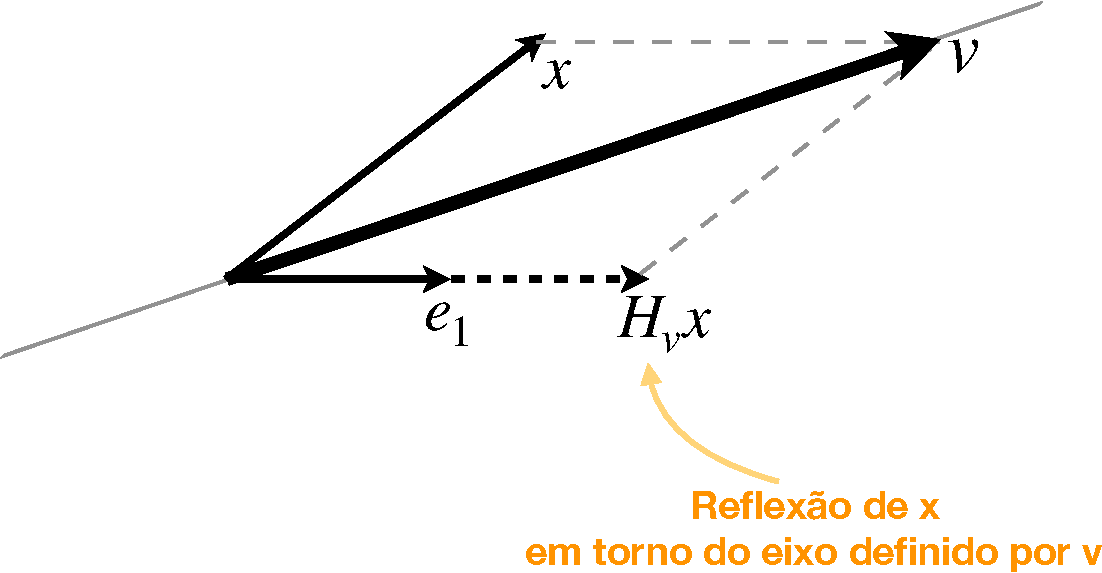
\includegraphics[scale=0.6]{figs/householder.pdf}
\end{center}

Para uma dada matriz $A$, tomando-se $x$ sua primeira coluna e $v$ como acima,
ent�o $H_v A$ vai zerar quase toda primeira coluna, que fica
\begin{equation}
  \begin{bmatrix}
    |x|\\
    \vdots\\
    0
  \end{bmatrix}.
\end{equation}

Continuando a multiplica��o � esquerda por rota��es Householder adequadas,
podemos triangular a matriz:
\begin{align}
  \tilde Q A &= R\\
  A &= \tilde Q^\top R = QR
\end{align}
que � a decomposi��o QR de $A$.

Tais matrizes Householder adequadas s�o da seguinte forma:
